\chapter{Introdução}

A introdução eu devo escrever por último, deve conter a importancia do projeto,
devo descrever o problema e a solução: "existe um problema e foi resolvido
assim". O final da introdução deve descrever a estrutura dos capitulos dando
uma pincelada rapida em cada um.

\chapter{Conceitos}
\section{Arquitetura de Software}
\section{Atributos de Modularidade}
\subsection{Acoplamento}
\subsection{Coesão}

\chapter{Implementação do Extrator}

Este projeto consiste na implementação de um novo extrator para o egypt onde a
análise seja feita direto do código fonte do sem necessidade de compilação, ou
seja, o novo extrator irá buscar as informações diretamente no código fonte sem
necessidade de usar o GCC ou qualquer outro compilador. Com isto será possível
analisar projetos que não compilem mais, seja por falhas no código ou por
possuir dependencias não satisfeitas. Além disto, este novo extrator trará mais
duas vantagens: primeiro, o tempo necessário para analisar um projeto cairá e
segundo, as informações obtidas serão mais precisas já que alguns dados
importantes não se perderão como acontece por exemplo com macros em projetos
C/C++ \cite{SourceVersusObjectCodeExtraction} que se perdem com o extrator
baseado em GCC.

\section{egypt}

O egypt foi originalmente desenvolvido por Andreas
Gustafsson\footnote{http://www.gson.org/egypt} com o objetivo de gerar gráficos
de chamada entre funções de programas escritos em C, ele funciona lendo os
arquivos intermediários gerados pelo GCC\sigla{GCC}{GNU C Compiler} e os
converte num gráfico de chamada no formato usado pelo
Graphviz\footnote{http://www.graphviz.org}, um programa para visualização de
gráficos.

O egypt é Software Livre e em Janeiro de 2009 começou a ser restruturado por
Antonio A S. Terceiro o qual o tem mantido
em\footnote{http://github.com/terceiro/egypt}. As principais mudanças sofridas
pelo egypt deste então foram \cite{StructuralComplexityEvolution}:

\begin{itemize}
\item Detecção de uso de variáveis, para identificar que função usa qual
variável.
\item Opção para agrupar chamada e uso de variaveis por módulo, com isto é
possível ter uma visão de dependência entre módulos.
\item Refatoração do script egypt em um design orientado a objetos, para
permitir diferentes módulos de extração e relatório.
\item Geração de relatório de métricas, como coesão e acoplamento por exemplo.
\end{itemize}

Segue abaixo como ficou estruturado o egypt após a refatoração:

\begin{description}
\item[egypt] Script principal
\item[Egypt::Extractor] Extrator baseado nos arquivos intermediários do GCC
\item[Egypt::Metrics] Gera relatório de métricas com os dados do Egypt::Model
\item[Egypt::Model] Armazena os dados obtidos pelo extrator
\item[Egypt::Output::DOT] Gera saída no formato do Graphviz com os dados de Egypt::Model
\end{description}

\section{Doxygen (e a sua API)}

Doxygen\footnote{http://www.doxygen.org} é um sistema de documentação para C++,
C, Java, Objective-C, Python, IDL, Fortran, VHDL, PHP e C\#. Com ele é possível
gerar documentação em HTML, RTF, PostScript, PDF, \LaTeX\ e man pages, ele
extrai a documentação existente no código fonte e também a partir deste mesmo
código ele extrai informações de hierarquia e colaboração entre os módulos do
projeto. É baseado nesta capacidade de extrair informações do código fonte que
o Doxygen foi escolhido como base para implementação deste novo extrator para o
egypt.

O Doxygen é Software Livre e está disponível sob a GPL\sigla{GPL}{GNU Public
License}v2 em
\footnote{https://doxygen.svn.sourceforge.net/svnroot/doxygen/trunk}, junto aos
fontes deste programa existe um pequeno exemplo chamado doxyapp, que foi usado
como base para este projeto, este exemplo implementa uma ferramenta para parsing de
código fonte bem próximo as necessidades deste projeto.

Entre as inúmeras classes presentes na API do Doxygen é importante destacar as
seguintes:

\begin{itemize}
\item Doxygen - Provê um namespace para varáveis e funções globais usadas pelo
doxygen
\item CodeOutputInterface - Interface de saída de trecho de código para os
parsers
\item MemberDef - Definição de um membro (símbolo) de classe
\item FileDef - Definição de um arquivo
\end{itemize}

O exemplo doxyapp utilizado como base para este projeto implementa a interface CodeOutputInterface disponível para
quem desejar escrever na saída gerada pelo Doxygen trechos de código extraido
dos fontes do projeto sendo analisado.

\section{Implementação do Extrator usando a API do Doxygen}

O Doxygen apesar de oferecer todos os recursos necessários para
analisar projetos C/C++ e extrair o uso de símbolos (funções, varáveis, etc)
que é o objetivo deste projeto, não possibilita que a saída gerada seja
customizada, apenas oferece opções específicas como PDF e HTML por exemplo. É
necessário então adaptar o Doxygen para gerar uma saída num formato
específico e apenas com as informações necessárias, para isto foi criado o
doxyparse, um parser capaz de analisar códigos C/C++ e possivelmente outras
linguagens suportadas pelo Doxygen, extraindo símbolos como variáveis e funções
com a identificação de onde são declarados e onde são utilizados.

Seguindo a interface CodeOutputInterface, a mesma utilizada no exemplo doxyapp,
foi possível reaproveitar no doxyparse todo o poder que o Doxygen fornece para
análise de código fonte e ainda gerar a saída da forma desejada.

O doxyparse então reaproveita os recursos existentes no Doxygen para fazer a
análise de código e gerar uma saída que será lida pelo extrator a ser
implementado no egypt, o doxyparse redefine algums parâmetros da configuração
do Doxygen para obter o comportamento desejado, como: analisar diretorios
recursivamente, não gerar saida em Latex ou HTML, extrair tanta informação
quanto possível do código fonte, extrair informação de chamada e não gerar
mensagens de warnings.

O doxyparse faz então a análise dos fontes de um diretorio ou arquivo(s)
passados como parâmetro via linha de comando e extrai destes fontes os simbolos
encontrados contendo a informação de onde são definidos e onde são usados. Após
isto é gerado uma saída num formato específico para ser depois analisado pelo
extrator implementado no egypt. Na figura~\ref{exemplo-saida-doxyparse} tem um
exemplo de saída gerado pelo doxyparse.

\begin{figure}[h]
\begin{Verbatim}[frame=single,fontsize=\relsize{-2},fontfamily=courier]
module module1.c
   function main in line 5
      uses function callback defined in module3.c
      uses function say_bye defined in module2.c
      uses function say_hello defined in module2.c
      uses variable variable defined in module3.c
\end{Verbatim}
\caption{exemplo de saída do doxyparse}
\label{exemplo-saida-doxyparse}
\end{figure}

Com a saída gerada pelo doxyparse o egypt precisa agora de um extrator que
entenda estes dados e gere a saída no formato do Graphviz que irá então gerar o
gráfico de chamada entre os módulos. O egypt já possui a infraestrutura
para gerar saída no formato do Graphviz, a classe Egypt::Output::DOT é a
responsável por isto, ela lê os dados armazenados em Egypt::Model e gera a
saída corretamente. O Egypt::Model é alimentado pelo extrator, que neste caso será
o Egypt::Extrator::Doxyparse.

O egypt em sua implementação atual possui somente a classe Egypt::Extractor que
faz a extração baseada nos arquivos intermediários gerados pelo GCC, para o
objetivo deste trabalho esta classe foi transformada numa implementação
genérica contendo apenas uma interface padrão para os extratores GCC e
Doxyparse. O extrator GCC é baseado no código já existente e o Doxyparse é um
novo extrator que usa como entrada os dados de saída do doxyparse. Na
figura~\ref{egypt-diagram-extractor} está o diagrama desta nova estrutura.

\begin{figure}[h]
\center
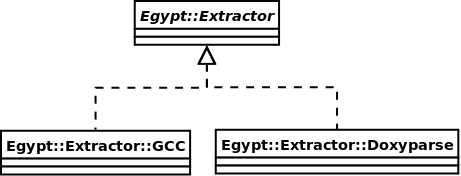
\includegraphics[scale=0.5]{imagens/egypt-diagram-extractor}
\caption{diagrama da hierarquia de classes do extrator do egypt}
\label{egypt-diagram-extractor}
\end{figure}

O egypt agora pode extrair informações usando 2 métodos diferentes. Um usando o
Egypt::Extractor::GCC que faz a extração baseada nos arquivos intermediários do
GCC e outro usando o Egypt::Extractor::Doxyparse que faz a análise utilizando o
doxyparse. Exemplo de execução do egypt usando cada um dos extratores:

\begin{Verbatim}[frame=single,fontsize=\relsize{-2},fontfamily=courier]
 $ egypt --extractor Doxyparse <arquivos>
 $ egypt --extractor GCC <arquivos>
\end{Verbatim}

\chapter{Avaliação}

Nos resultados eu posso comparar o que consegui com a nova ferramenta comparado ao modo antigo do egypt extrair informacoes.

\section{Procedimento}

Com o extrator Doxyparse pronto é necessário eleger algum projeto que tenha o
código fonte disponível para fazer a análise de extração de informações de
colaboração entre módulos, o projeto escolhido foi o
ristretto\footnote{http://goodies.xfce.org/projects/applications/ristretto}, um
Software Livre escrito em C para visualização de imagens no ambiente Desktop
Xfce\footnote{http://www.xfce.org}, este mesmo projeto foi utilizado por
\cite{StructuralComplexityEvolution} onde foram gerados dados de dependencia
entre módulos para as versões 0.0.1 até a 0.0.21 usando o antigo
extrator baseado em GCC. Foi gerado os mesmos dados utilizando o extrator
Doxyparse e então comparados aos dados extraidos pelo extrator GCC.

\section{Resultados}

http://gitorious.org/doxygen

Os resultados obtidos foram satisfatórios e atingiram o objetivo inicial que
foi possibilitar estração de dados sem necessidade de compilar o software em
questão, contudo algumas diferenças entre o extrator original do egypt e o
atual baseado no Doxyparse foram notadodas. Nas figuras \ref{ristretto-0.0.1},
\ref{ristretto-0.0.11} e \ref{ristretto-0.0.21} estão gráficos de chamadas
entre módulos das versões 0.0.1, 0.0.11 e 0.0.21 do ristretto gerado pelo egypt
usando o extrator Doxyparse e o GCC :

\begin{figure}
\center
\subfigure[ristretto-0.0.1-doxyparse][Egypt::Extrator::Doxyparse]{
   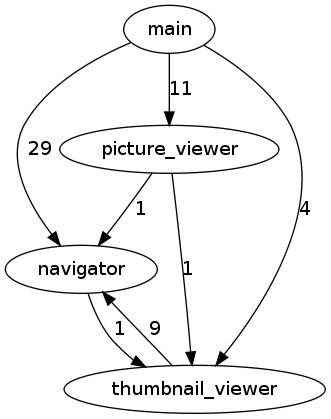
\includegraphics[scale=0.5]{imagens/ristretto-0_0_1-doxyparse}
}
\qquad
\subfigure[ristretto-0.0.1-gcc][Egypt::Extrator::GCC]{
   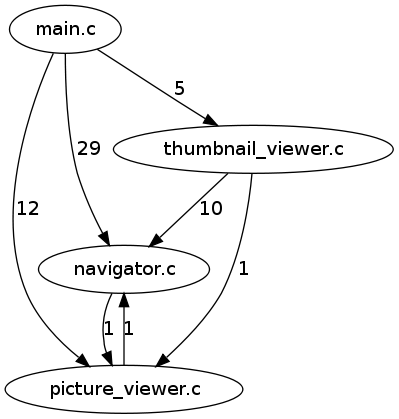
\includegraphics[scale=0.5]{imagens/ristretto-0_0_1-gcc}
}
\caption{gráfico de chamada entre módulos do {\bf Ristretto 0.0.1} gerado pelo Egypt}
\label{ristretto-0.0.1}
\end{figure}

Na figura~\ref{ristretto-0.0.1} nota-se uma diferença interessante entre as
informaçõe extraídas pelo GCC e o Doxyparse, há uma inversão entre os módulos
thumbnailer\_viewer e picture\_viewer. Enquanto o Doxyparse diz que o
picture\_viewer chama o thumbnailer\_viewer no GCC temos o contrário, qual
deles está errado ou os dois estão errados?

\begin{figure}
\center
\subfigure[ristretto-0.0.11-doxyparse][Egypt::Extrator::Doxyparse]{
   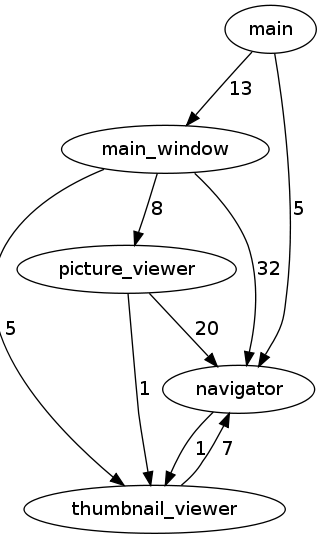
\includegraphics[scale=0.5]{imagens/ristretto-0_0_11-doxyparse}
}
\qquad
\subfigure[ristretto-0.0.11-gcc][Egypt::Extrator::GCC]{
   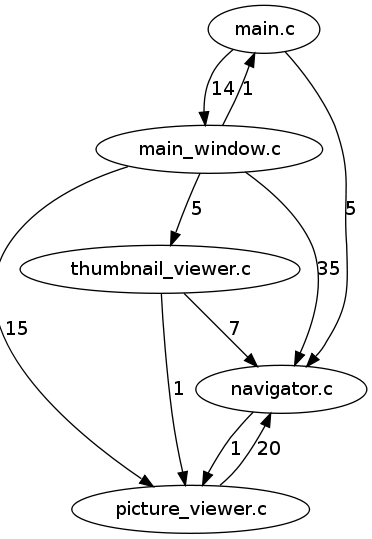
\includegraphics[scale=0.5]{imagens/ristretto-0_0_11-gcc}
}
\caption{gráfico de chamada entre módulos do {\bf Ristretto 0.0.11} gerado pelo Egypt}
\label{ristretto-0.0.11}
\end{figure}

O mesmo ocorre nas figuras \ref{ristretto-0.0.11} e \ref{ristretto-0.0.21}, mas
nestas outras ainda temos mais observações, por exemplo na
figura~\ref{ristretto-0.0.11} o GCC diz que o módulo main\_window chama main,
já no Doxyparse não há esta chamada.

\begin{figure}
\center
\subfigure[ristretto-0.0.21-doxyparse][Egypt::Extrator::Doxyparse]{
   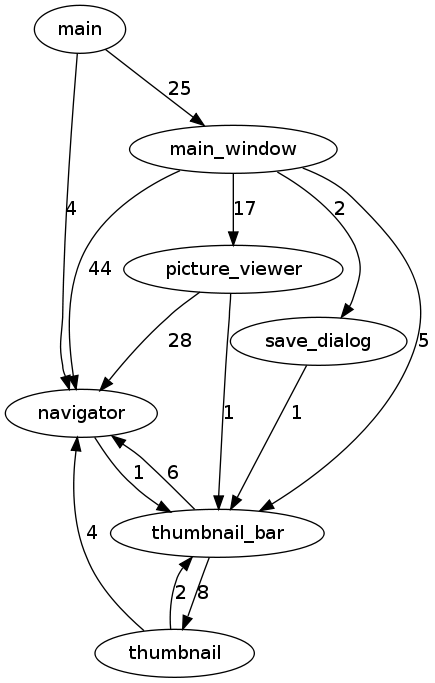
\includegraphics[scale=0.5]{imagens/ristretto-0_0_21-doxyparse}
}
\qquad
\subfigure[ristretto-0.0.21-gcc][Egypt::Extrator::GCC]{
   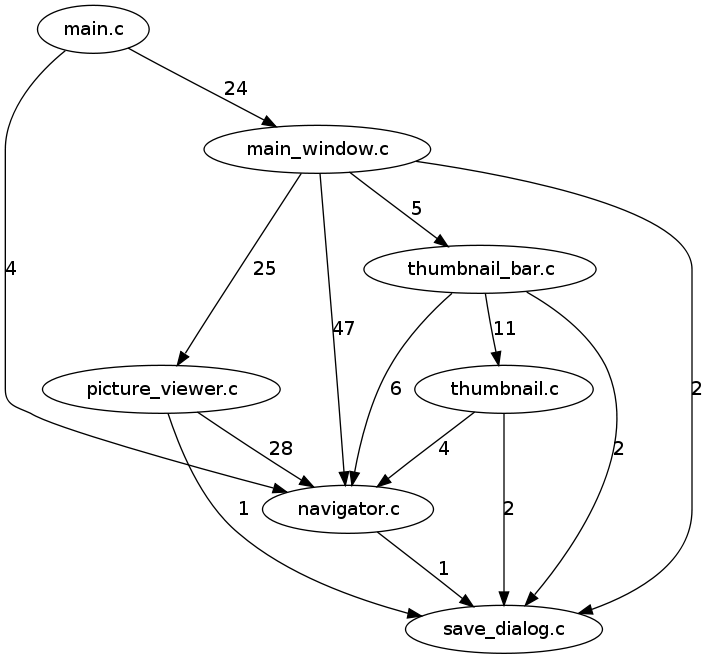
\includegraphics[scale=0.5]{imagens/ristretto-0_0_21-gcc}
}
\caption{gráfico de chamada entre módulos do {\bf Ristretto 0.0.21} gerado pelo Egypt}
\label{ristretto-0.0.21}
\end{figure}

Na figura~\ref{ristretto-0.0.21} temos ainda outra importante, o GCC nos diz
que o módulo save\_dialog é chamado por vários módulos: main\_window,
thumbnail, navigator, picture\_viewer e thumbnail\_bar sendo que não faz
sentido já que este é um módulo que encapsula a exibição de uma caixa de
diálogo onde teoricamente deveria ser chamada apenas pelos módulos que compõe a
interface, como diz o Doxyparse que apenas main\_window chama save\_dialog, mas
o Doxyparse dá uma informação controversa onde o save\_dialog chama
thumbnail\_bar e isto pode não ser verdade (verificar).

Ainda sobre a análise do ristretto-0.0.21 a saída gerada pelo doxyparse
confunde o uso do simbolo parent\_class que é uma variavei estática definida
por todos os módulos, mas o Doxygen registra este símbolo relacionado ao
primeiro módulo que ele analisa, e nos demais módulos que fazem uso dele o
Doxygen acha que o módulo está usando o simbolo definido no primeiro modulo
analisado. Isto foi solucionado ignorando as chamadas aos simbolos estaticos
fora do módulo sendo analisado, ou seja, só se considera chamada a símbolos
estaticos se eles estiverem no módulo que o simbolo foi encontrado.

\section{Discussão}

\chapter{Conclusão}

A conclusão eu devo escrever por último, deve conter algo assim: "Este trabalho
tinha objetivo tal e atingiu tal objetivo". Deve ter referencia de como foi
feito e se os resultados foram bons, medios, satisfatorios, ruins, etc. E ao
final deve ter trabalhos futuros que eu tenha interesse ou não de fazer.

Trabalhos futuros: verificar Natural Docs, semelhando ao Doxygen implementado
em Perl e suporta outras linguagens.
